
%%%%%%%%%%%%%%%%%%%%%%%%%%%%%%%%%%%%%
% [x] Removed we
% [x] Tidied up language

\paragraph{Slow Host Code}
The program is now using an SoA format. The runtimes, however, are unexpected: the time to run 128x128 and 128x256 are almost equal, similarly with 256x256 and 1024x1024. It would be expected that the time of the first size would be noticeably faster, especially in the latter case. After investigating further why this may be the case, one suspicion could be that the host code is slowing down the execution of the program rather than kernels. 

The runtime of the host code can be tested, by removing all computation from the kernels. If the program still runs with similar runtimes, it would suggest that the host code is slowing down the program. The times generated from this experiment, can be seen in Table~\ref{table:commented-kernels}. 


\begin{table}[ht]
\vspace{-5mm}
\centering
\caption{Runtimes after removing the computation}
\vspace{1mm}
\begin{tabular}{|c||p{5.8em}|}
    \hline
    Size & Runtime (s) \\
    \hline
    128x128 & 1.922 \\
    \hline
    256x256 & 3.887 \\
    \hline
    1024x1024 & 3.036 \\
    \hline
\end{tabular}
\label{table:commented-kernels}
\vspace{-3mm}
\end{table}

These results are not below the ballpark times given. This would suggest that the host code could be optimised further. This leads to the question: \textit{Is enqueuing kernels an expensive operation? If it is can it be optimised in some way?} After experimenting with the queuing of kernels one thing becomes apparent. There is a linear relationship between the number of arguments and the time needed to queue them. This can be seen in Figure~\ref{graph:slow-host-kernel-args-scaling}. This effect is noticed when the arguments are buffers much sooner than if the arguments are integers. Therefore, it would make sense to try to minimise the number of arguments to a kernel that are buffers.



\begin{figure}[ht]
% This file was created by tikzplotlib v0.9.1.
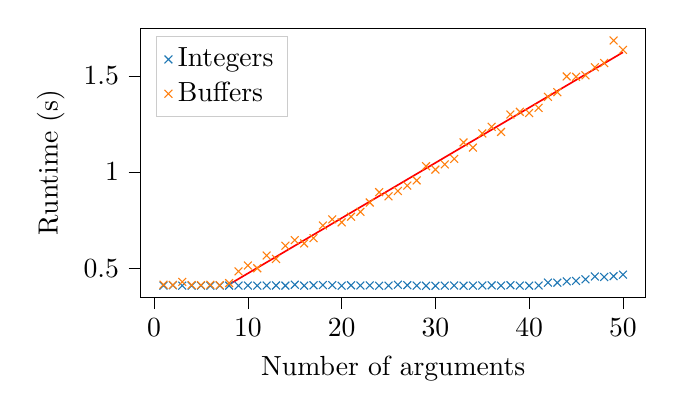
\begin{tikzpicture}

\definecolor{color0}{rgb}{0.12156862745098,0.466666666666667,0.705882352941177}
\definecolor{color1}{rgb}{1,0.498039215686275,0.0549019607843137}

\begin{axis}[
height=5cm,
width=8cm,
legend cell align={left},
legend style={fill opacity=0.8, draw opacity=1, text opacity=1, at={(0.03,0.97)}, anchor=north west, draw=white!80!black},
tick align=outside,
tick pos=left,
x grid style={white!69.0196078431373!black},
xlabel={Number of arguments},
xmin=-1.45, xmax=52.45,
xtick style={color=black},
y grid style={white!69.0196078431373!black},
ylabel={Runtime (s)},
ymin=0.34797581, ymax=1.74823159,
ytick style={color=black}
]
\addplot [only marks, mark=x, draw=color0, fill=color0, colormap/viridis]
table{%
x                      y
1 0.408938
2 0.411233
3 0.408951
4 0.408869
5 0.409075
6 0.408630
7 0.409599
8 0.409134
9 0.409537
10 0.409541
11 0.409010
12 0.409656
13 0.410045
14 0.409219
15 0.413942
16 0.409022
17 0.410913
18 0.412203
19 0.411667
20 0.408739
21 0.410963
22 0.409593
23 0.410292
24 0.408464
25 0.409441
26 0.413967
27 0.411422
28 0.409200
29 0.408387
30 0.408280
31 0.409054
32 0.409923
33 0.408738
34 0.409158
35 0.409863
36 0.410641
37 0.409353
38 0.411392
39 0.409373
40 0.408952
41 0.409714
42 0.424751
43 0.424433
44 0.431163
45 0.433972
46 0.441783
47 0.456787
48 0.454138 
49 0.458432
50 0.466376
};
\addlegendentry{Integers}
\addplot [only marks, mark=x, draw=color1, fill=color1, colormap/viridis]
table{%
x                      y
1 0.413959
2 0.412788
3 0.428915
4 0.4122962
5 0.4116238
6 0.4138856
7 0.4118764
8 0.4223356
9 0.4834678
10 0.5140242
11 0.4996726
12 0.5657012
13 0.5479644
14 0.6168688
15 0.6458056
16 0.6287808
17 0.6560834
18 0.721907
19 0.7539046
20 0.7383354
21 0.767807
22 0.7929246
23 0.8415554
24 0.8955696
25 0.8736594
26 0.9015882
27 0.9296822
28 0.956363
29 1.0304728
30 1.0127568
31 1.039857
32 1.06864
33 1.1539132
34 1.127261
35 1.2007254
36 1.235649
37 1.2087534
38 1.2992762
39 1.3135694
40 1.3071474
41 1.3338828
42 1.3911198
43 1.415439
44 1.4975512
45 1.4955442
46 1.5030964
47 1.5450664
48 1.5672718
49 1.6845836
50 1.6357272
};
\addlegendentry{Buffers}

\addplot [semithick, red]
table {%
8 0.415357330655391
9 0.444106986892178
10 0.472856643128964
11 0.501606299365751
12 0.530355955602537
13 0.559105611839324
14 0.58785526807611
15 0.616604924312897
16 0.645354580549683
17 0.67410423678647
18 0.702853893023256
19 0.731603549260043
20 0.760353205496829
21 0.789102861733615
22 0.817852517970402
23 0.846602174207188
24 0.875351830443975
25 0.904101486680761
26 0.932851142917548
27 0.961600799154334
28 0.990350455391121
29 1.01910011162791
30 1.04784976786469
31 1.07659942410148
32 1.10534908033827
33 1.13409873657505
34 1.16284839281184
35 1.19159804904863
36 1.22034770528541
37 1.2490973615222
38 1.27784701775899
39 1.30659667399577
40 1.33534633023256
41 1.36409598646934
42 1.39284564270613
43 1.42159529894292
44 1.4503449551797
45 1.47909461141649
46 1.50784426765328
47 1.53659392389006
48 1.56534358012685
49 1.59409323636364
50 1.62284289260042
};

\end{axis}

\end{tikzpicture}

\vspace{-3mm}
\caption{Time to queue 50000 kernels with n arguments.}
\label{graph:slow-host-kernel-args-scaling}
\vspace{-3mm}
\end{figure}

